This is about the smartcitizen CO results.

One SmartCitizen CO sensor was tested against the EPA reference.  It was 1 month old at the time of installation, and ran for 52 days (from 4/15 - 6/6 2016) with two ~40 minute service interruptions.  This test gave 74,961 samples of minute resolution data.


\subsection{Pre-processing}

Talk about process for taking raw aux/working electrodes and making the basic calibration data.


\begin{figure}[htb]
 	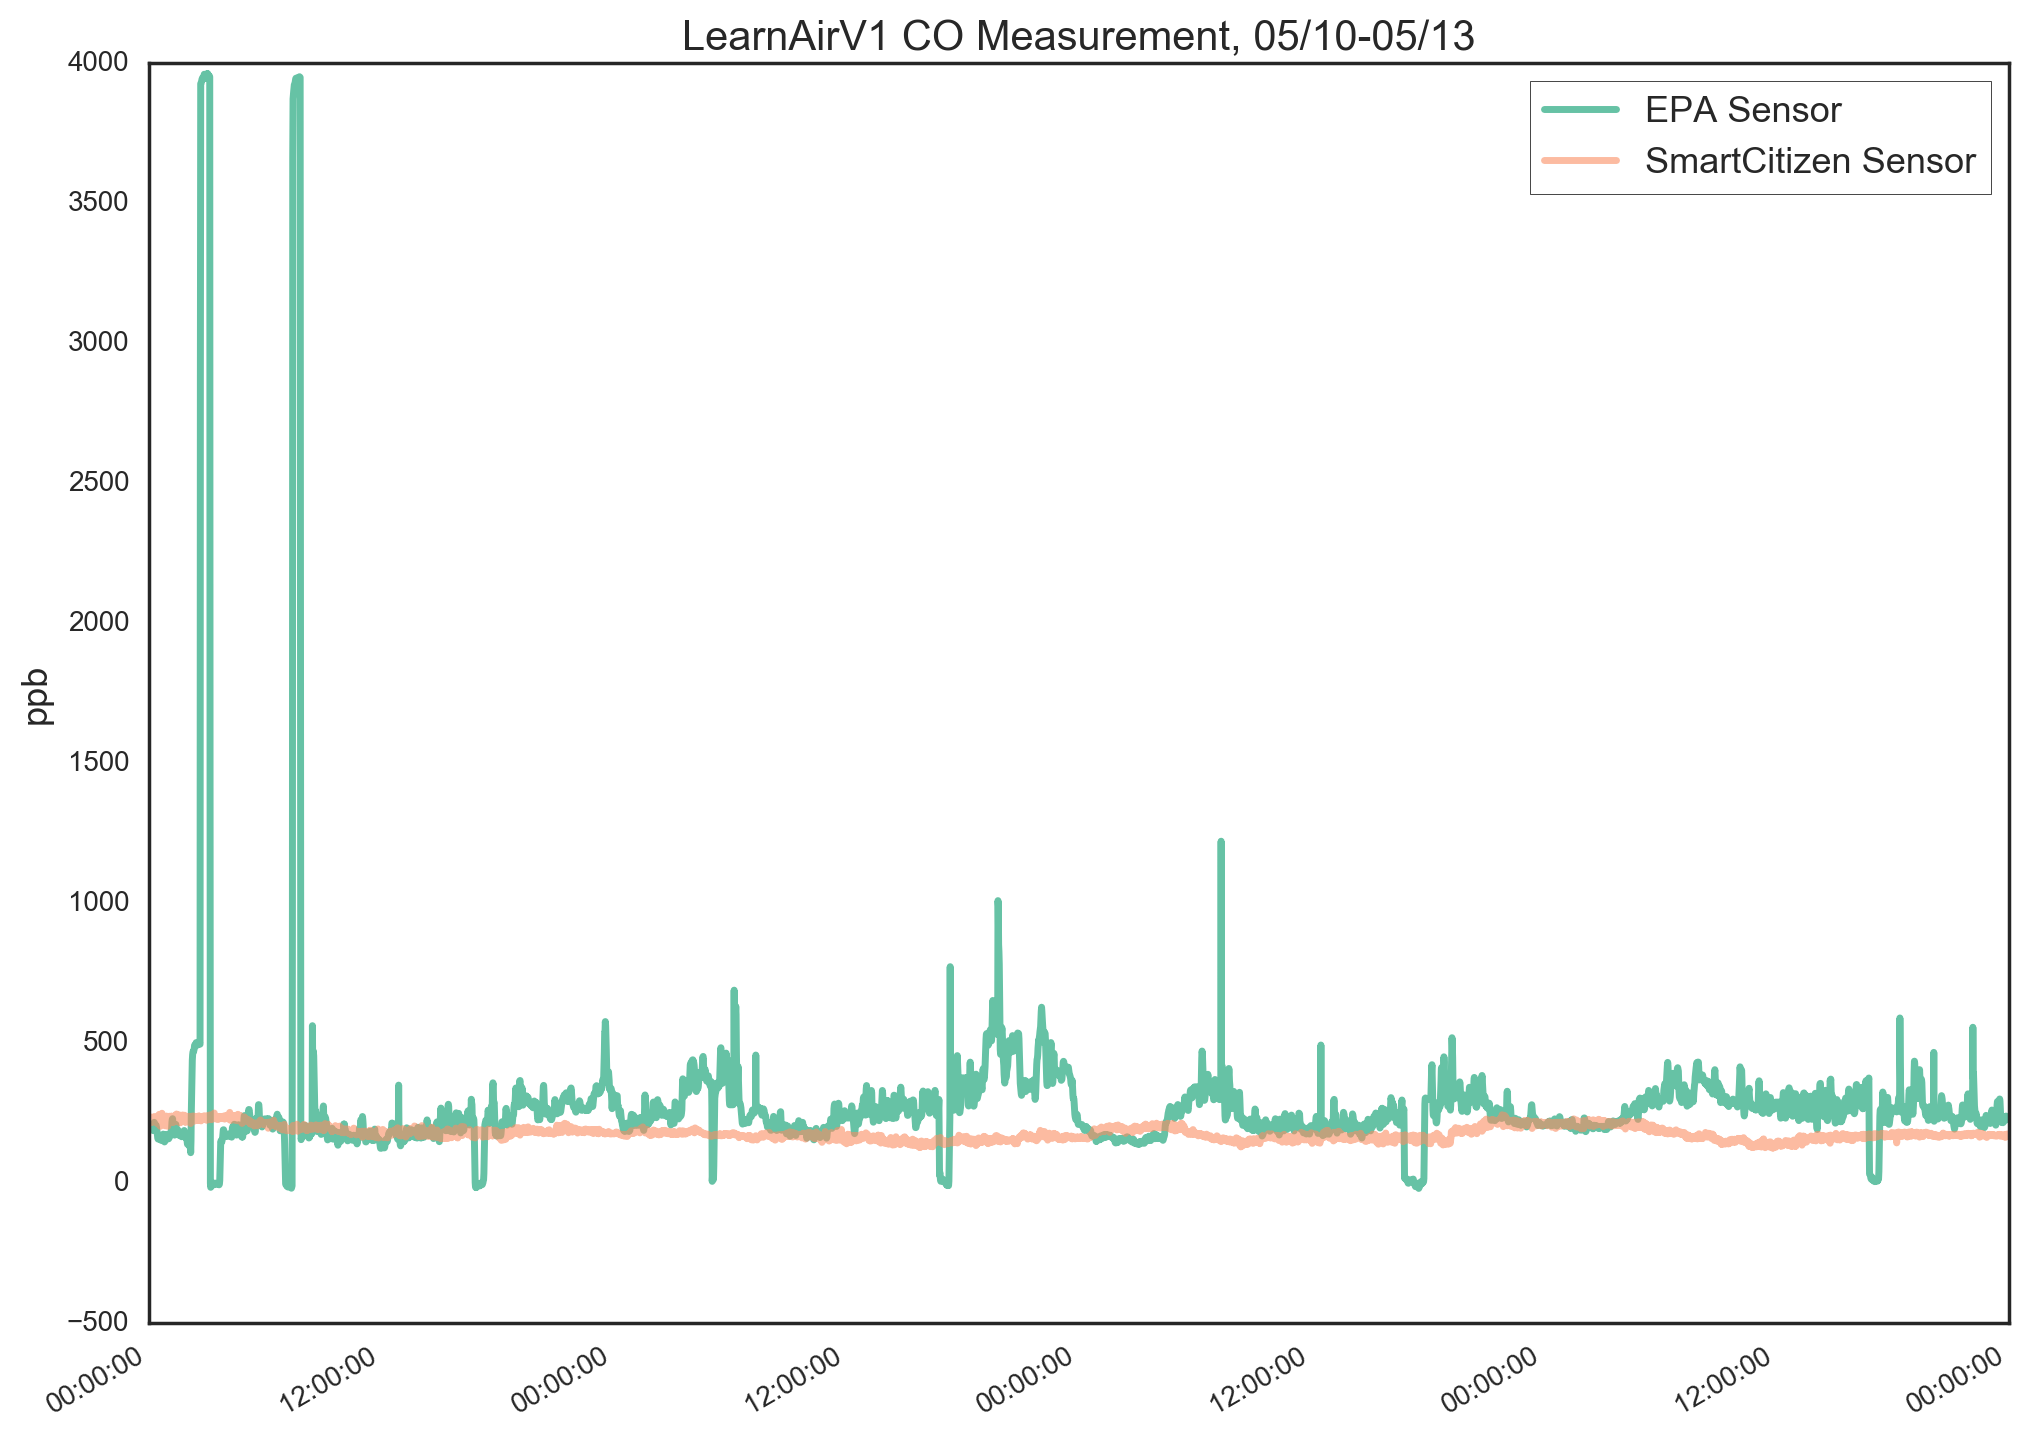
\includegraphics[width=\textwidth]{figs/co_sck_zoomed}               
 	 \caption{SmartCitizen CO Raw Data}
  	\label{fig:sck_co_raw_zoomed}
\end{figure}


\begin{figure}[htb]
 	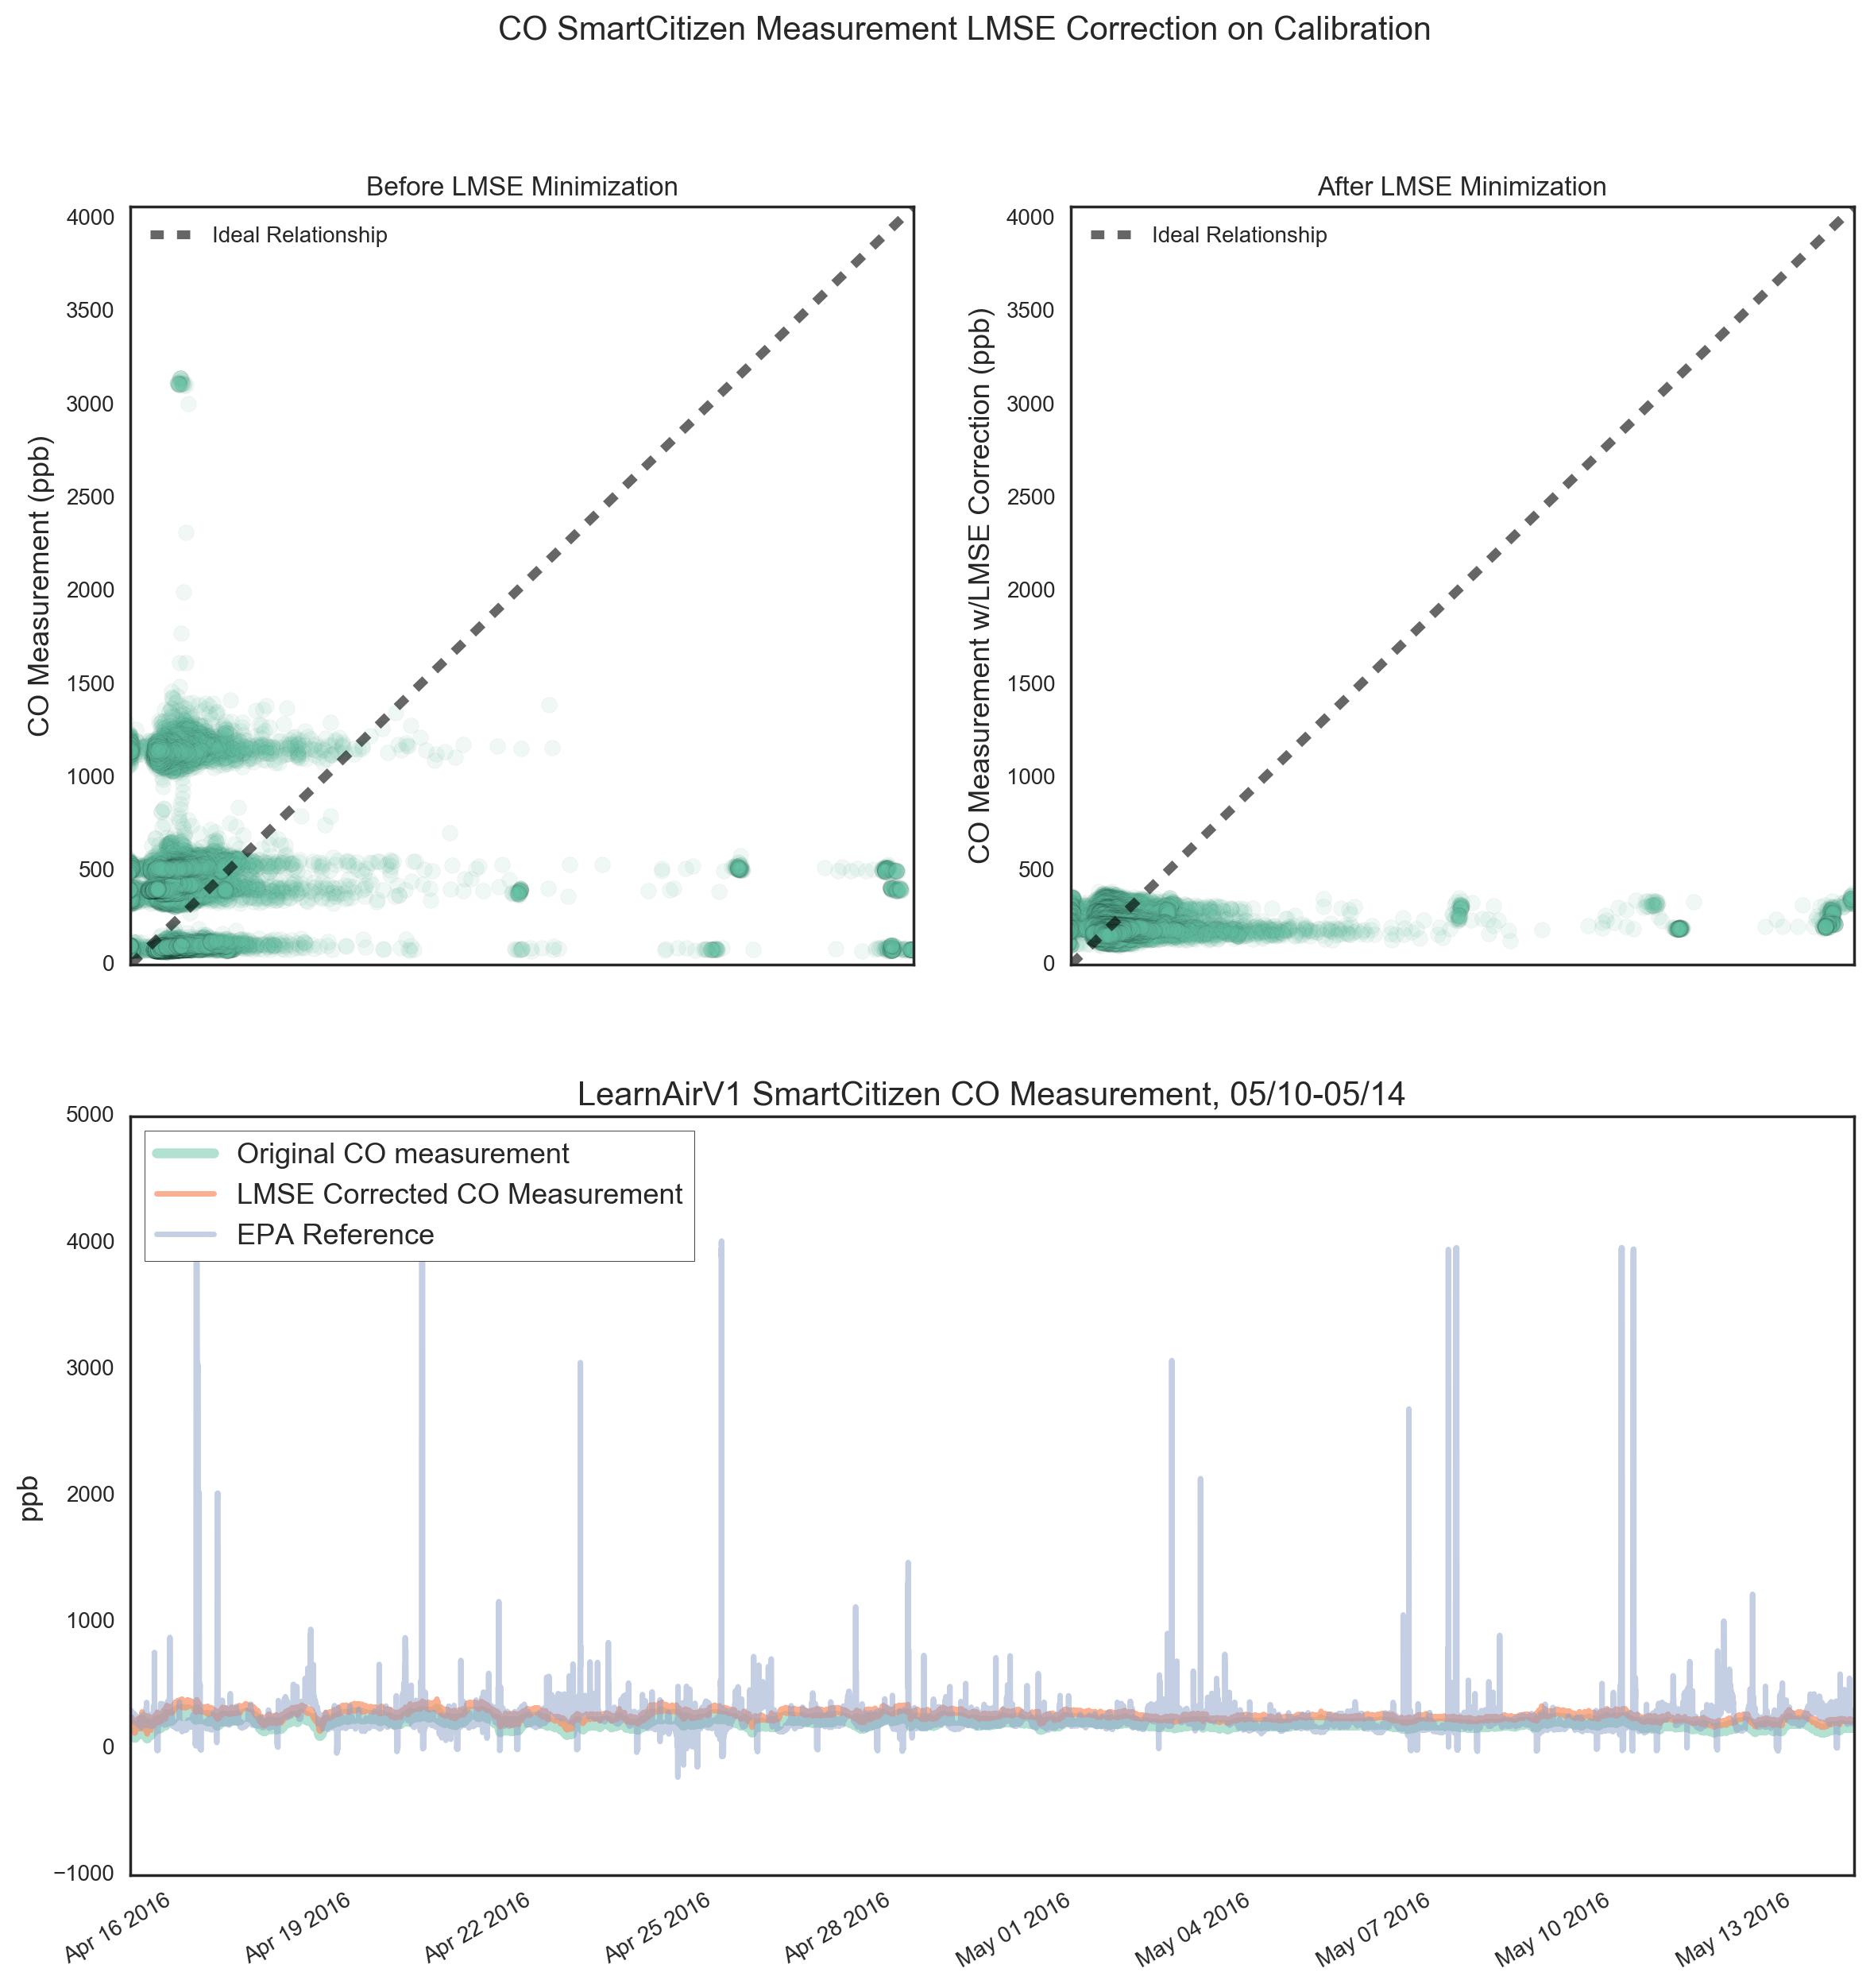
\includegraphics[width=\textwidth]{figs/sck_co_lmse}               
 	 \caption{SmartCitizen CO after LMSE Calibration}
  	\label{fig:sck_co_lmse}
\end{figure}








\subsection{Machine Learning}


\begin{figure}[htb]
 	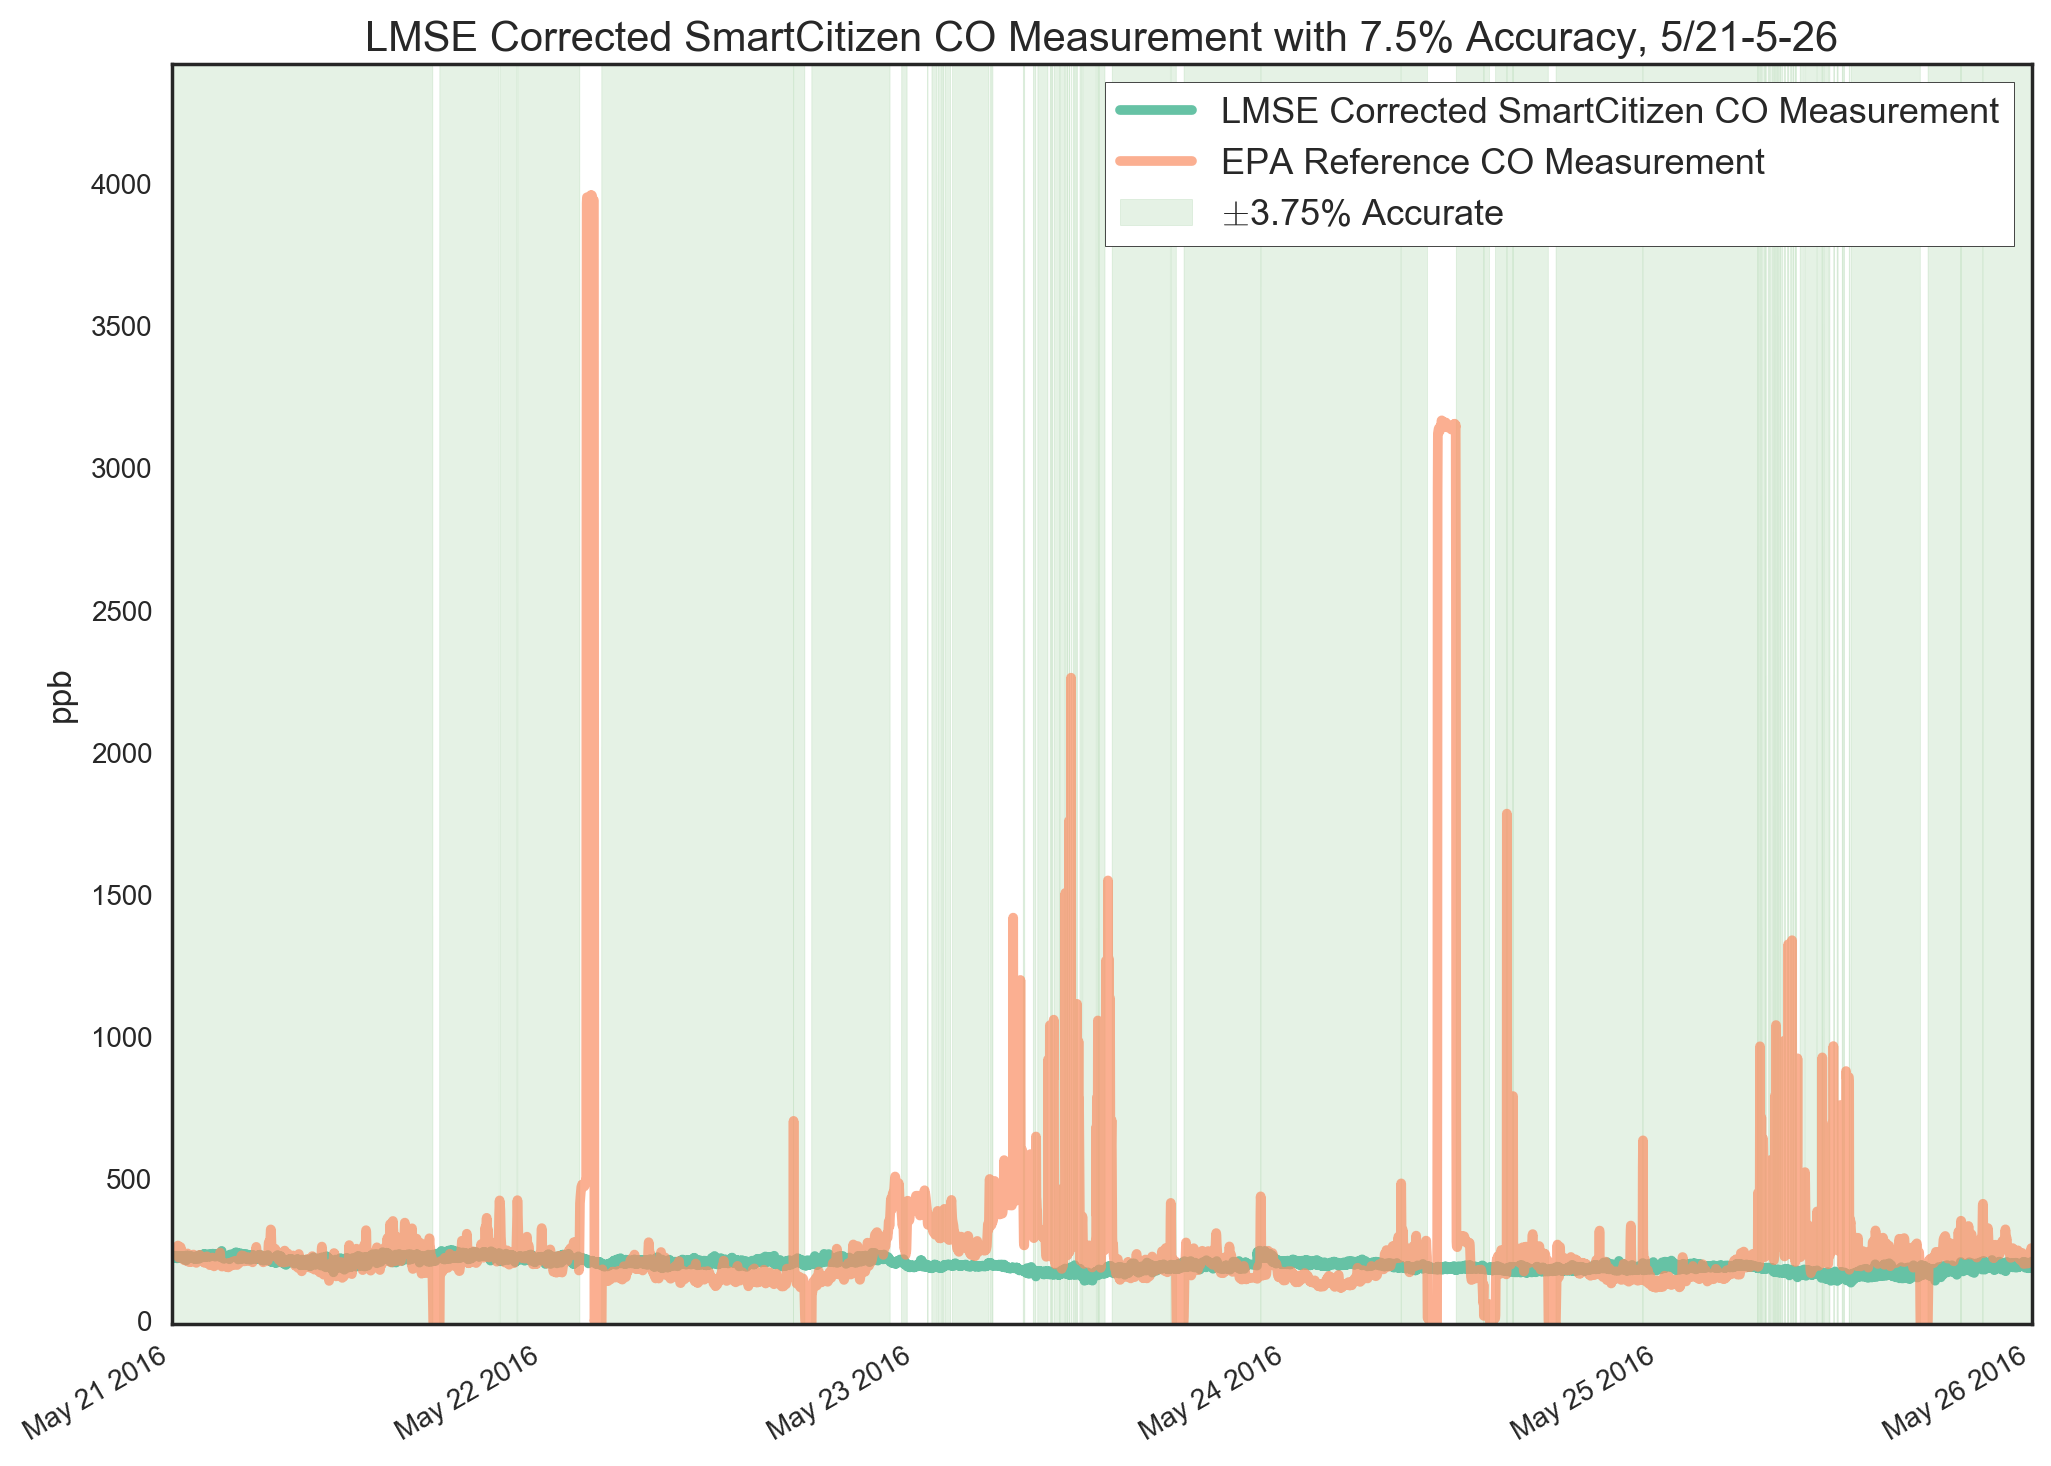
\includegraphics[width=\textwidth]{figs/sck_co_with_7p5_accuracy_zoomed}               
 	 \caption{SmartCitizen CO with 7.5\% Accuracy Threshold}
  	\label{fig:sck_co_with_7p5_accuracy_zoomed}
\end{figure}

\begin{figure}[htb]
 	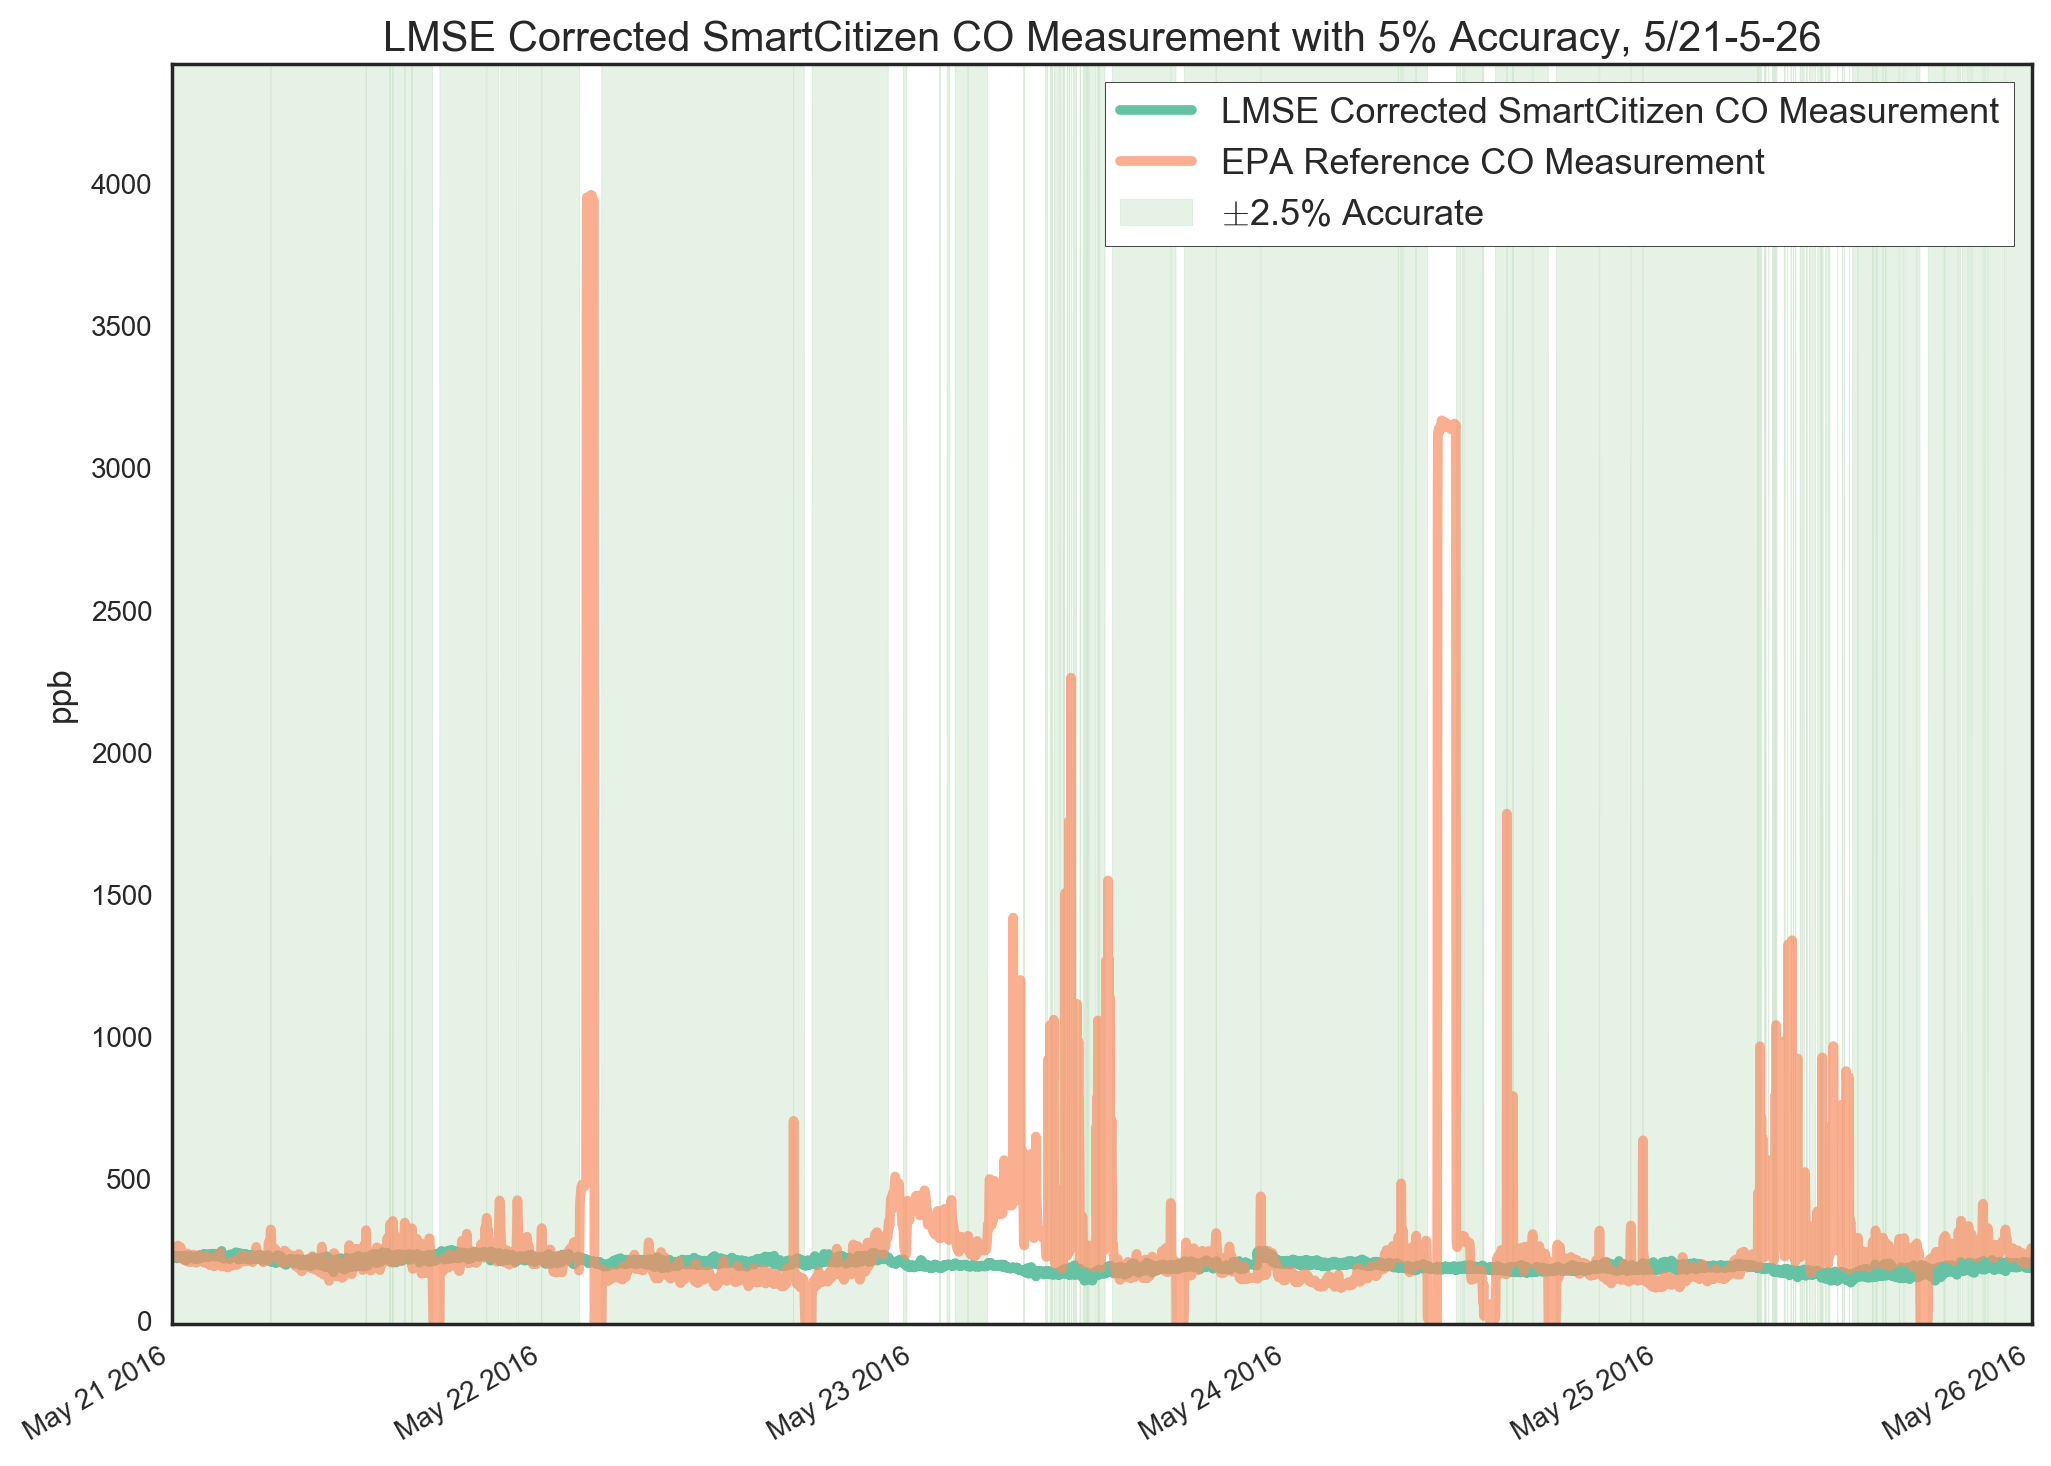
\includegraphics[width=\textwidth]{figs/sck_co_with_5_accuracy_zoomed}               
 	 \caption{SmartCitizen CO with 5\% Accuracy Threshold}
  	\label{fig:sck_co_with_5_accuracy_zoomed}
\end{figure}




parameters = {'C':[0.001, 0.1, 10, 1000], 'penalty':('L1', 'L2') }, 2 fold

===== best ROC\_AUC score 0.81902438871

===== best params {'penalty': 'L1', 'C': 10}



\begin{table}[H]
\centering
\begin{tabular}{|c|c|c|c|c|}
\toprule
\multicolumn{5}{|c|}{Error Rates for SmartCitizen CO with Logistic Regression} \\
&\multicolumn{2}{|c|}{all features} & \multicolumn{2}{|c|}{top 15 features} \\
&shuffled & chunked & shuffled & chunked \\
avg & 0.09 & 0.09 & 0.09 & 0.09 \\
min & 0.08 & 0.03 & 0.09 & 0.08 \\
max & 0.09 & 0.12 & 0.09 & 0.11 \\
\bottomrule
\end{tabular}
\label{tab:sck_co_error_rates}
\caption{Error Rates for Predicting SmartCitizen CO Accuracy with Logistic Regression}
\end{table}



\begin{table}[H]
\centering
\offinterlineskip
\hspace*{-5cm}\raisebox{-3.5cm}[0pt][0pt]{\rotatebox[origin=c]{90}{\parbox[c][0pt][c]{3cm}{\textbf{Actual Values}\\[20pt]}}}\par
\hspace*{1cm}\MyHBox[\dimexpr5.1cm+6\fboxsep\relax]{Predicted Values}\par
\hspace*{1cm}\MyHBox{0}\MyHBox{1}\par
\MyTBox{0}{197.0}{1187.4}
\MyTBox{1}{108.6}{13499.2}
}
\label{tab:as1_co_confusion}
\caption{Average SmartCitizen CO Confusion Matrix w/Shuffled K-Fold}
\end{table}


\begin{figure}[htb]
 	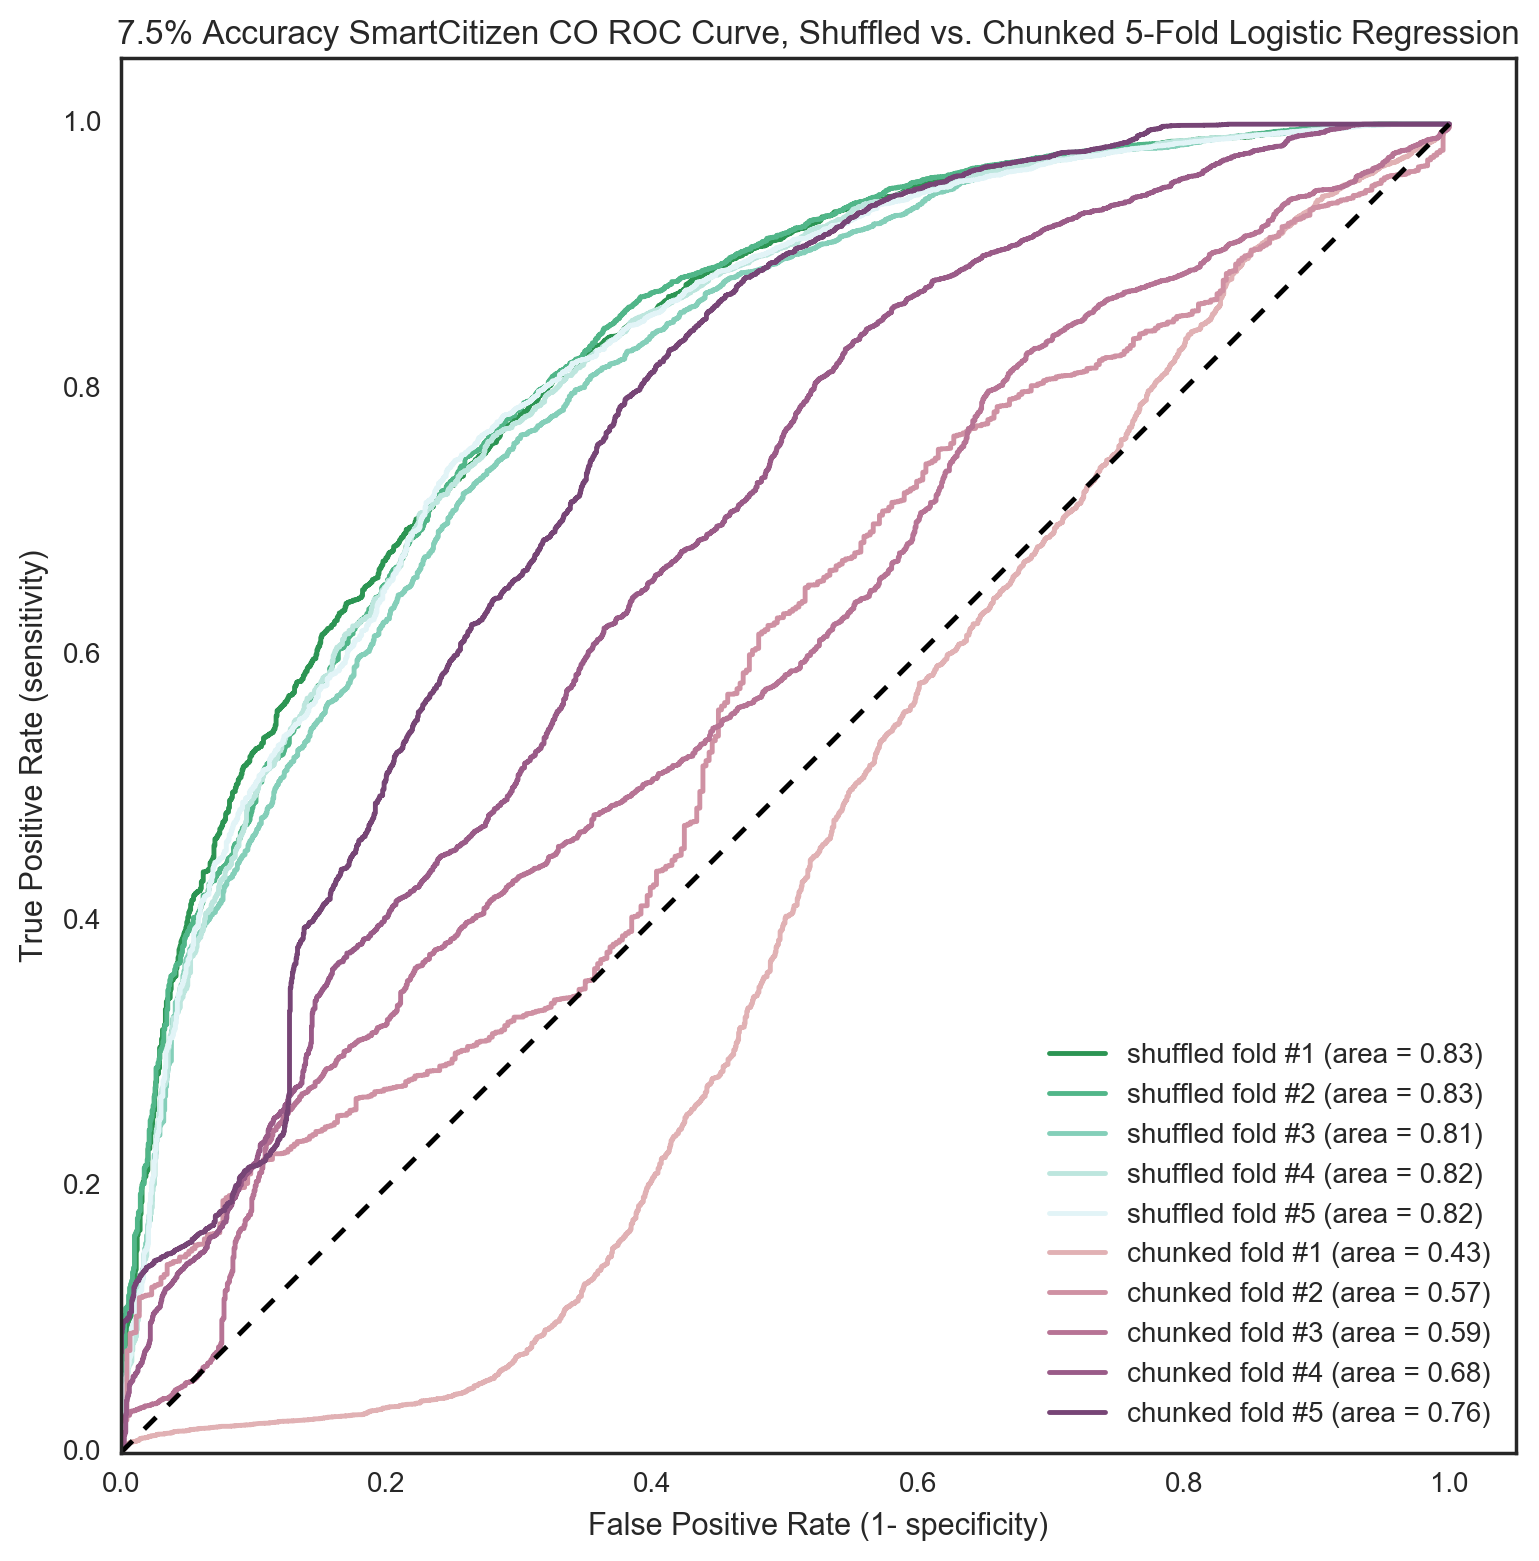
\includegraphics[width=\textwidth]{figs/sck_co_7p5_roc}               
 	 \caption{SmartCitizen CO ROC Curve}
  	\label{fig:sck_co_7p5_roc}
\end{figure}


here's text referencing the (Table \ref{tab:as1_co_randomforest_features}).

\begin{table}[H]
\centering
\begin{tabular}{lllllllll}
\\
\\
\toprule
Feature & Importance \\
\midrule
bkcarbon &  0.027481618644 \\
avg\_60\_bkcarbon &  0.0265308524121 \\
avg\_720\_bkcarbon &  0.0231734007362 \\
avg\_1440\_bkcarbon &  0.0213230536622 \\
avg\_60\_forecastio\_windSpeed &  0.0155772873357 \\
min\_since\_plugged\_in &  0.0151174982516 \\
temp\_sck\_box\_differential &  0.0148499597107 \\
avg\_60\_forecastio\_windBearing &  0.014573874136 \\
daily\_avg\_forecastio\_humidity &  0.0145367615821 \\
avg\_60\_forecastio\_dewPoint &  0.0138511147354 \\
avg\_60\_forecastio\_pressure &  0.0138476329536 \\
daily\_avg\_sck\_temperature &  0.0138353139286 \\
avg\_30\_ws &  0.0136031033823 \\
daily\_avg\_sck\_humidity &  0.0135231176757 \\
avg\_720\_lmse\_scaled\_sharpDust &  0.0132885608127 \\
\bottomrule
\end{tabular}
\label{tab:as1_co_randomforest_features}
\caption{Top 15 Features from Random Forest for SmartCitizen CO, used in Pruned Logistic Regression}
\end{table}



\begin{figure}[htb]
 	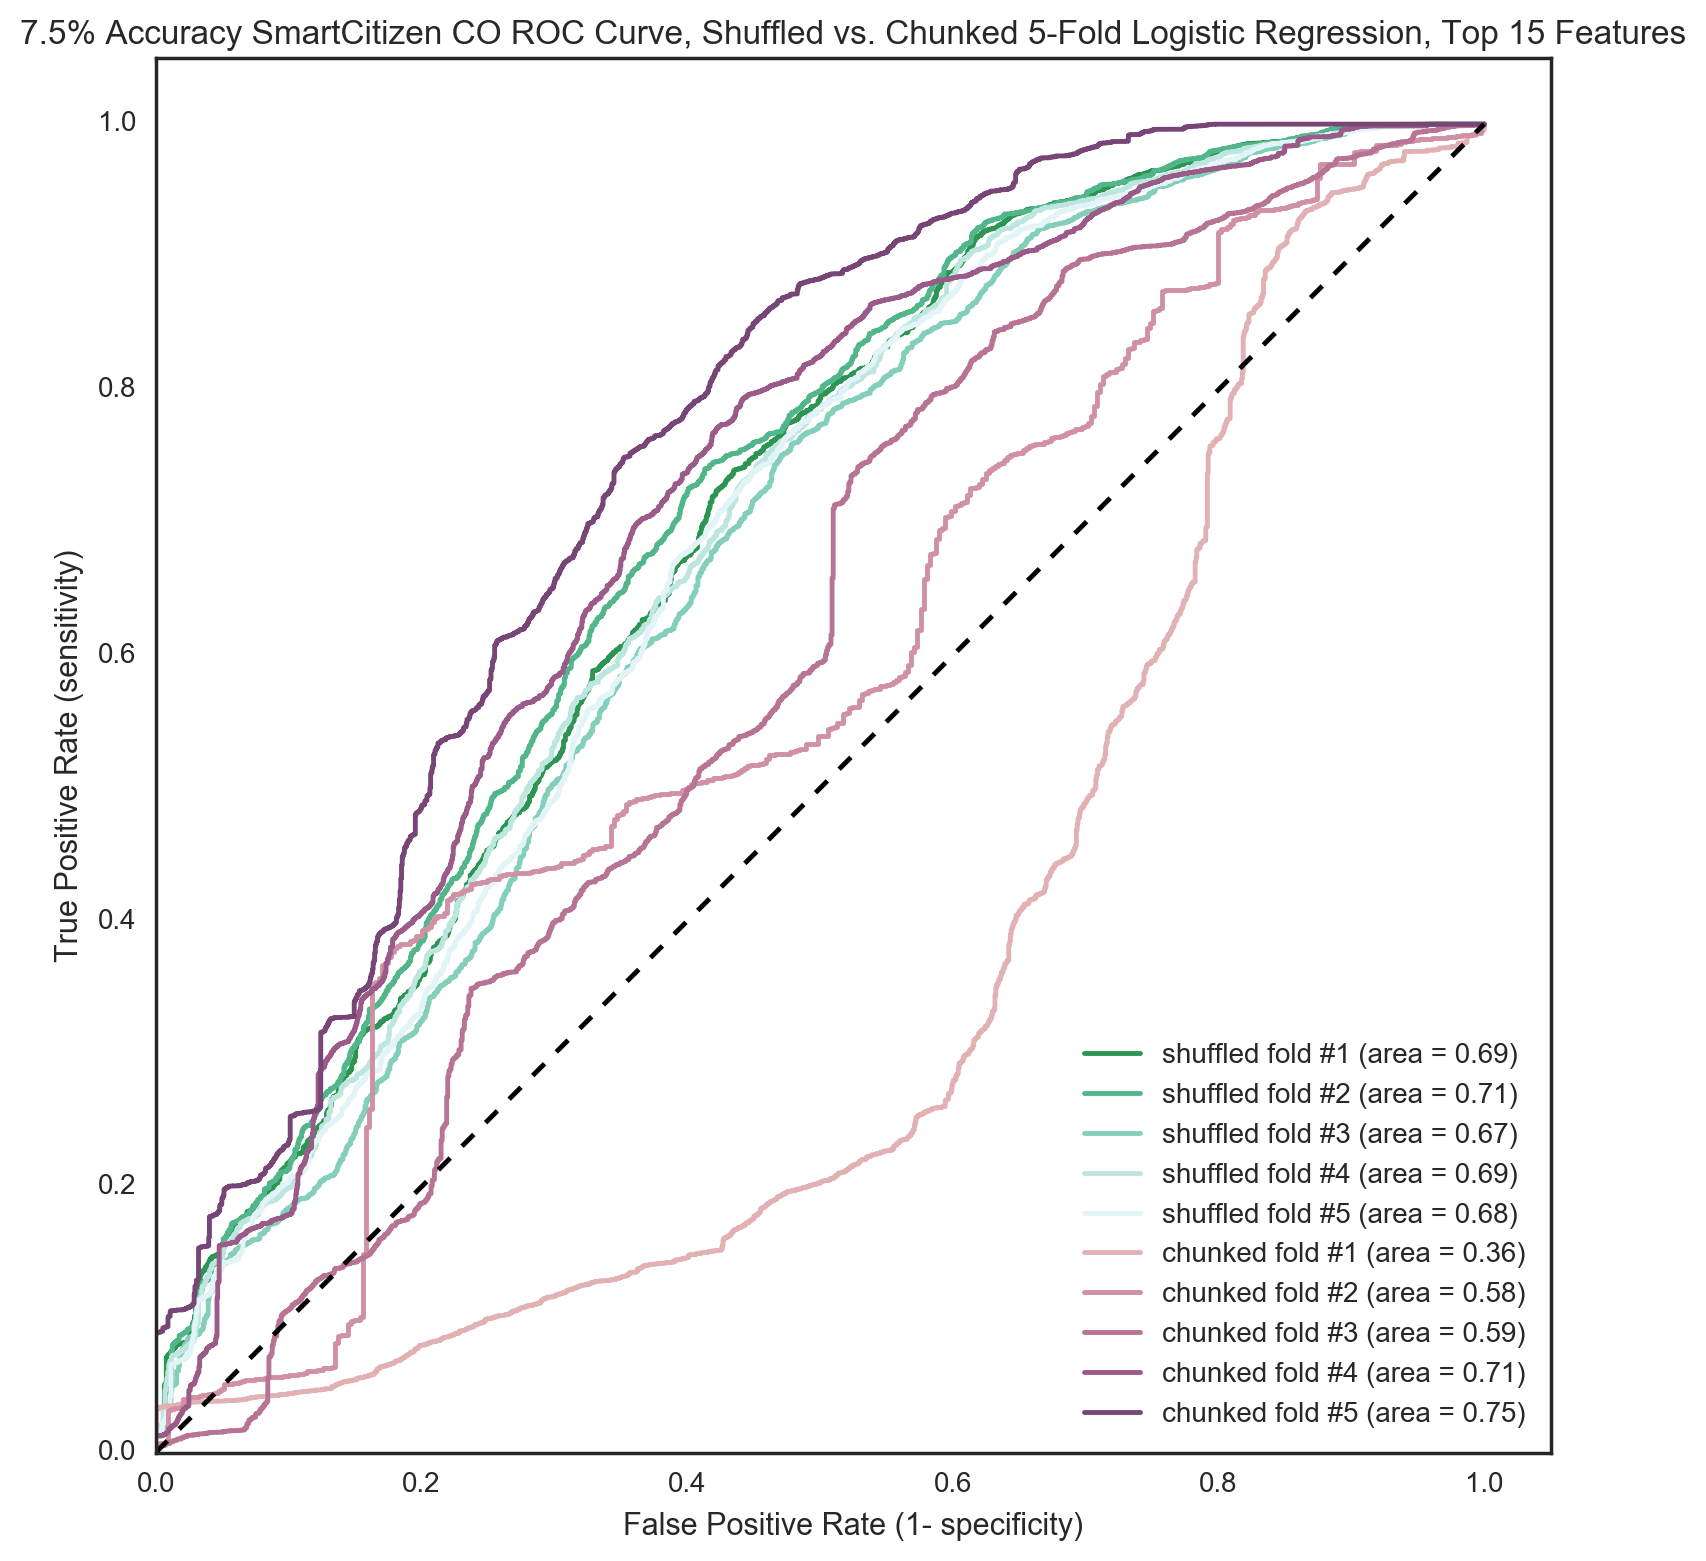
\includegraphics[width=\textwidth]{figs/sck_co_7p5_roc_pruned_features}               
 	 \caption{SmartCitizen CO ROC Using Top 15 Features}
  	\label{fig:sck_co_7p5_roc_pruned_features}
\end{figure}

\begin{figure}[htb]
 	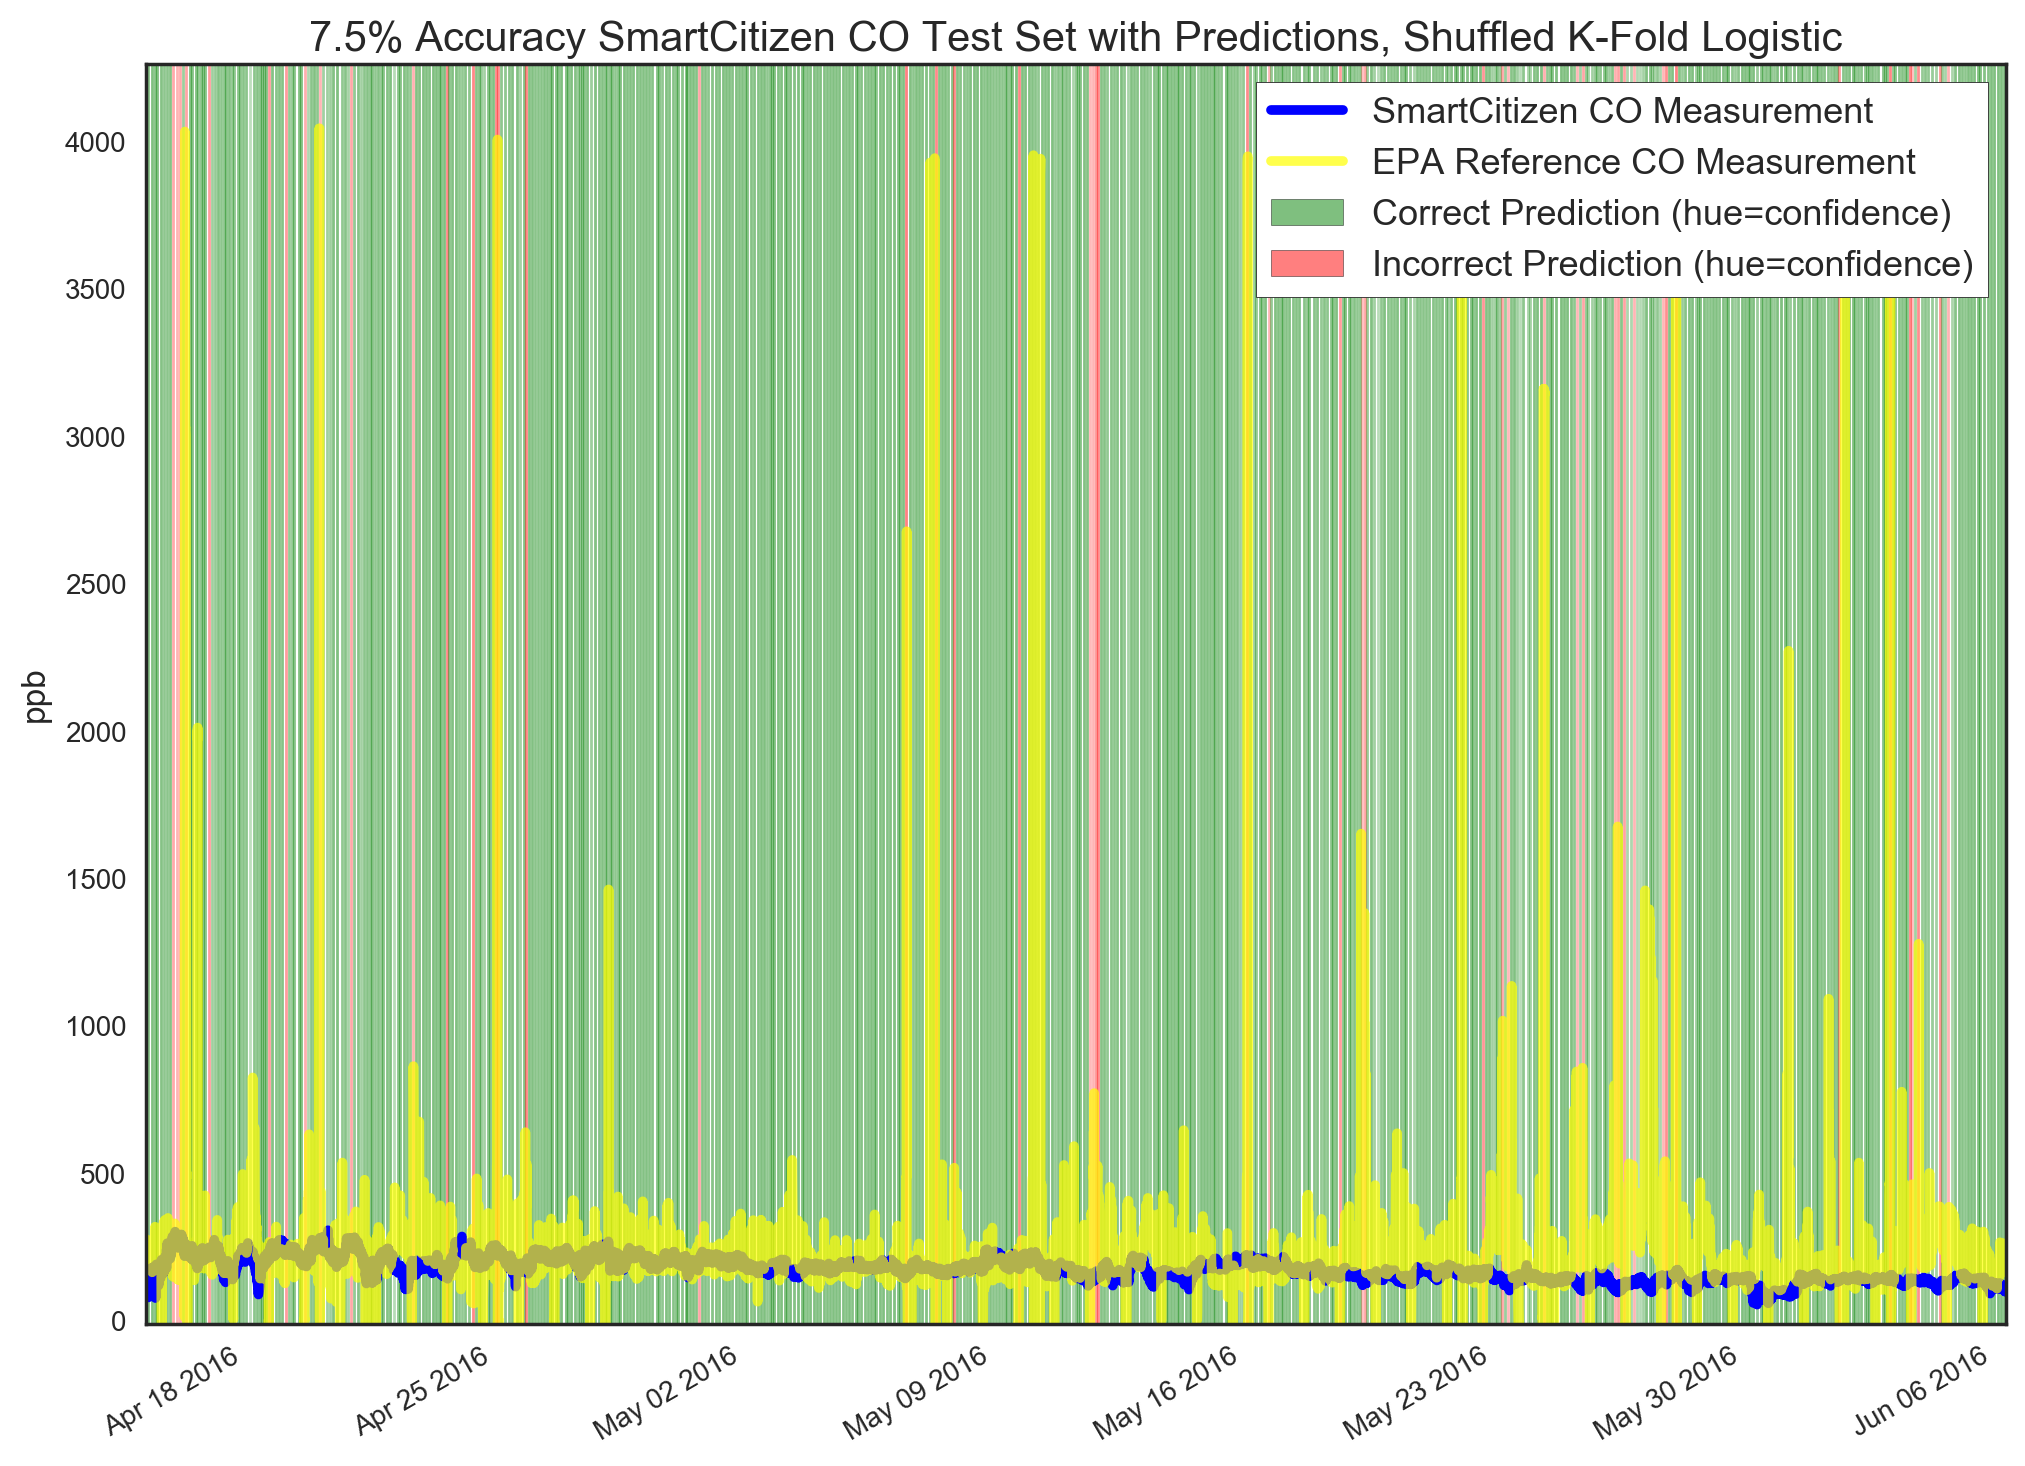
\includegraphics[width=\textwidth]{figs/sck_co_7p5_logistic_predictions}               
 	 \caption{SmartCitizen CO Prediction Accuracy}
  	\label{fig:sck_co_7p5_logistic_predictions}
\end{figure}



here's text referencing the (Table \ref{tab:as1_co_top_features}).

\begin{table}[H]
\centering
\begin{tabular}{lllllllll}
\\
\\
\toprule
     & Corr. & Lasso & Lin Reg & RF   & RFE  & Ridge & Stability & Mean \\
\midrule
bkcarbon                            & 1     & 0          & 0    & 1    & 0.58  & 0.28      & 0.93 & 0.54 \\
avg\_60\_bkcarbon                   & 0.98  & 0          & 0    & 0.25 & 0.53  & 0.15      & 0.83 & 0.39 \\
evening                             & 0.17  & 0          & 0.07 & 0.19 & 0.82  & 0.18      & 1    & 0.35 \\
avg\_1440\_bkcarbon                 & 0.57  & 0          & 0    & 0.37 & 0.53  & 0.44      & 0.54 & 0.35 \\
humidity\_box\_differential         & 0.1   & 0          & 0.01 & 0.22 & 1     & 1         & 0.02 & 0.34 \\
afternoon                           & 0.17  & 0          & 0.07 & 0    & 0.84  & 0.19      & 1    & 0.32 \\
avg\_60\_forecastio\_humidity       & 0.01  & 0          & 0.01 & 0.12 & 1     & 1         & 0    & 0.31 \\
temp\_sck\_box\_differential        & 0.09  & 0          & 0    & 0.45 & 0.84  & 0         & 0.73 & 0.3  \\
Solar Panel ( V)                    & 0.05  & 0          & 1    & 0    & 0.77  & 0         & 0    & 0.26 \\
avg\_720\_bkcarbon                  & 0.65  & 0          & 0    & 0.26 & 0.27  & 0.14      & 0.43 & 0.25 \\
forecastio\_apparentTemperature     & 0.04  & 1          & 0    & 0.03 & 0.16  & 0         & 0.43 & 0.24 \\
lmse\_avg\_30\_scaled\_arduino\_ws  & 0     & 0          & 0    & 0.05 & 0.8   & 0.03      & 0.79 & 0.24 \\
forecastio\_clear-night             & 0     & 0          & 0.08 & 0.04 & 0.91  & 0.06      & 0.51 & 0.23 \\
forecastio\_partly-cloudy-day       & 0.06  & 0          & 0.08 & 0    & 0.91  & 0         & 0.55 & 0.23 \\
forecastio\_partly-cloudy-night     & 0.01  & 0          & 0.08 & 0    & 0.89  & 0.06      & 0.54 & 0.23 \\
avg\_30\_scaled\_arduino\_ws        & 0     & 0          & 0.02 & 0.07 & 0.81  & 0         & 0.74 & 0.23 \\
Noise ( mV)                         & 0.02  & 0          & 0    & 0.11 & 0.39  & 0.02      & 0.92 & 0.21 \\
avg\_720\_lmse\_scaled\_sharpDust   & 0.03  & 0          & 0    & 0.15 & 0.55  & 0.22      & 0.52 & 0.21 \\
derivative\_avg\_720\_bkcarbon      & 0     & 0          & 0    & 0.12 & 0.63  & 0.25      & 0.45 & 0.21 \\
daily\_avg\_sck\_humidity           & 0.07  & 0          & 0    & 0.18 & 0.59  & 0.17      & 0.4  & 0.2  \\
derivative\_avg\_360\_lmse\_as\_no2 & 0     & 0          & 0    & 0.11 & 0.55  & 0.73      & 0    & 0.2  \\
derivative\_avg\_1440\_bkcarbon     & 0.02  & 0          & 0    & 0.14 & 0.64  & 0.02      & 0.58 & 0.2  \\
evening\_rush                       & 0.13  & 0          & 0    & 0.04 & 0.49  & 0.1       & 0.54 & 0.19 \\
avg\_60\_forecastio\_pressure       & 0.07  & 0          & 0    & 0.26 & 0.41  & 0.01      & 0.6  & 0.19 \\
\bottomrule
\end{tabular}
\label{tab:as1_co_top_features}
\caption{Top Features for Predicting SmartCitizen CO}
\end{table}

